\section{Set Theory Basics}
For now, we will begin by giving an informal definition of sets to explore the basic ways that these mathematical objects interact.
As we should have already seen in the previous chapter, the idea of a \textit{set} or \textit{collection} arises very naturally in mathematics and logic.
For this reason, many regard the set as the most fundamental concept in all mathematics.

At the most foundational level, a \textit{set} is a mathematical object that contains other mathematical objects.
Now, although most sets of students encounter in high school math consist of just numbers, this doesn't necessarily have to case; in fact, sets can contain anything from functions, matrices, equations, or even sets themselves.\footnote{
I should note here that this idea of self-containment can be a source of great contradiction if not correctly managed. We will demonstrate this when we introduce set theory from a more formal approach.}

A convention that many mathematicians imply is to denote sets with \textit{capital letters}, so using this convention, we can give the following examples of sets
\begin{equation}
	A = \{1, a, b\},
\end{equation}
\begin{equation}
	B = \{f(x)=x^2+2, g(x)=3x+2, +\footnotemark\},
\end{equation}
\footnotetext{The \textit{plus} sign is \textit{technically} a mathematical object (more specifically a function of two variables), thus, there is nothing wrong with including it in a set.}
where the elements of the sets are denoted between the curly braces.

Now, I've given examples of \textit{finite sets}, but as we will see, \textit{finiteness} is certainly \textit{not} a requirement for a collection to be a set.

\subsection{Notation}
To make talking about sets easier, we will introduce the following notion as seen in \cref{fig:set-notation}.
\begin{figure*}[h]
	\centering
	\begin{tabular}{| c | m{6cm} |}
		\hline
		Symbol & Meaning \\
		\hline
		$\in,\notin$   & in and not in, respectively	\\
		\hline
		$\subset, \subseteq$ & proper subset, subset \\
		\hline
		$\not\subset, \not\subseteq$ & negations of above\\
		\hline
		$=$ & equivalent \\
		\hline
		$\cup$ & Union \\
		\hline
		$\cap$ & Intersect \\
		\hline
		$A^c$ & Compliment of $A$\\
		\hline
		$\setminus$ & Set difference \\
		\hline
		$\varnothing$ & Empty set, a set with no elements.\footnotemark\\
		\hline
	\end{tabular}
	\caption{}
	\label{fig:set-notation}
\end{figure*}
\footnotetext{Some texts commonly use the term \textit{null set} for an empty set, but the term \textit{null set} is also commonly used in math to refer to something completely different, so we will be solely using the term \textit{empty set} in this text.}

These symbols can be broken down into two main categories: The relational operators and the logical operators.
We will discuss them separately, but we will start with the relation operators.

The relational operators denote relationships between sets and can be understood by the direct English translations.
Many times, math symbols are created to shorthand English words, and as such, a way to understand and unravel the meaning behind these symbols is to translate them to the specific English words that they represent.

For example, we can interpret the phrase $x\in X$ to be \textit{$x$ in $X$} or \textit{$x$ is an element of $X$}.
By adding a slash through it, $x\notin X$ becomes the negation of the above, hence we have \textit{$x$ is not in $X$}.

Similarly, $X\subseteq Y$ and $X\not\subseteq Y$ can be understood as
\textit{$X$ is a subset of $Y$} and \textit{$X$ is not a subset of $Y$} respectively.
A set is a subset of a larger set if all of its components are included within the larger set, as seen in \cref{fig:subset}.
\begin{figure}[h]
	\centering
	\resizebox{0.3\linewidth}{!}{
	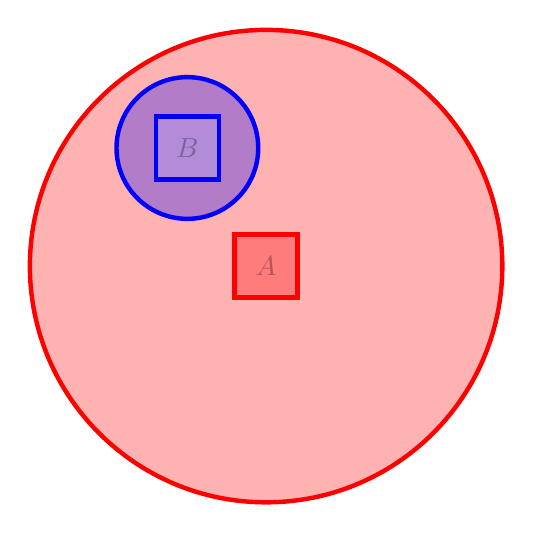
\begin{tikzpicture}
		\draw[ultra thick, draw=red, fill=red, fill opacity=.3] (0,0) circle (3)
			node[black,draw=red, fill=red, minimum size=0.8cm] {$A$};
		\draw[ultra thick, draw=blue, fill=blue, fill opacity=.3] (-1,1.5) circle (0.9)
			node[black,draw=blue, fill=blue!30, minimum size=0.8cm] {$B$};
	\end{tikzpicture}}
	\caption{Here we claim $B\subset A$}
	\label{fig:subset}
\end{figure}

Like how the $=$ is normally used in math, $A=B$ implies $A$ and $B$ are the same set.

Apart from $\in, \notin$, we can also give formal definitions of these symbols, shown as follows

\begin{define}
	$A\subseteq B$ if and only if for every $a\in A$, $a\in B$

	Similarly, $A\not\subseteq B$ if and only if there exists $a\in A$ such that $a\notin B$.
\end{define}

Notice, with these definitions, $A\subseteq A$ is a true statement, meaning a set is always a subset of itself.
Sometimes, to clarify that a subset is strictly smaller than the parent, we introduce the symbols $\subset$ and $\not\subset$ to denote \textit{proper subset} and \textit{not a proper subset} respectively.
A proper subset differs from a normal subset in the fact that proper subsets must not be equal to their parent; hence, we can give the following definitions:

\begin{define}
	$A \subset B$ if and only if $A\subseteq B$ and $A\neq B$.

	$A \not\subset B$ if and only if $A\not\subseteq B$ or $A\neq B$.
\end{define}

It turns out, when defining the \textit{equality} operator, we can characterize these using the subset operators.
To claim that two sets are equal is to claim that any element in either set is also in the other.
In other words,
\begin{equation}
	x\in A \text{ if and only if } x \in B.
\end{equation}
One can check that this characterization is equivalent to
\begin{equation}
	A\subseteq B \text{ and } B\subseteq A.
\end{equation}
Using this characterization, one arrives at the following:
\begin{define}
	$A=B$ if and only if $A\subseteq B$ and $B\subseteq A$.
\end{define}

Now, we can move on to the logical operators of set theory.
As one might expect, these operators are very much related to the logical operators that we saw in the previous chapter.
Unlike the relational operators, logical operators give a means to generate new sets, much like how addition and subtraction operators work with traditional arithmetic.

We start with \textit{union} and \textit{intersection} operators, which are the set-theoretic disjunction and conjunction operators.
As such, we can give the following definitions:
\begin{define}
	Let $A$ and $B$ be arbitrary sets, then $x\in A\cup B$ if and only if $x\in A$ or $x\in B$.
	\label{def:union}
\end{define}
\begin{define}
	Let $A$ and $B$ be arbitrary sets, then $x\in A\cap B$ if and only if $x\in A$ and $x\in B$.
	\label{def:intersect}
\end{define}

\cref{fig:union} shows the intersection and union operators as a Venn diagram, where the entire Venn diagram represents the union of $A$ and $B$.
\begin{figure}[h]
\centering
\resizebox{0.6\linewidth}{!}{
	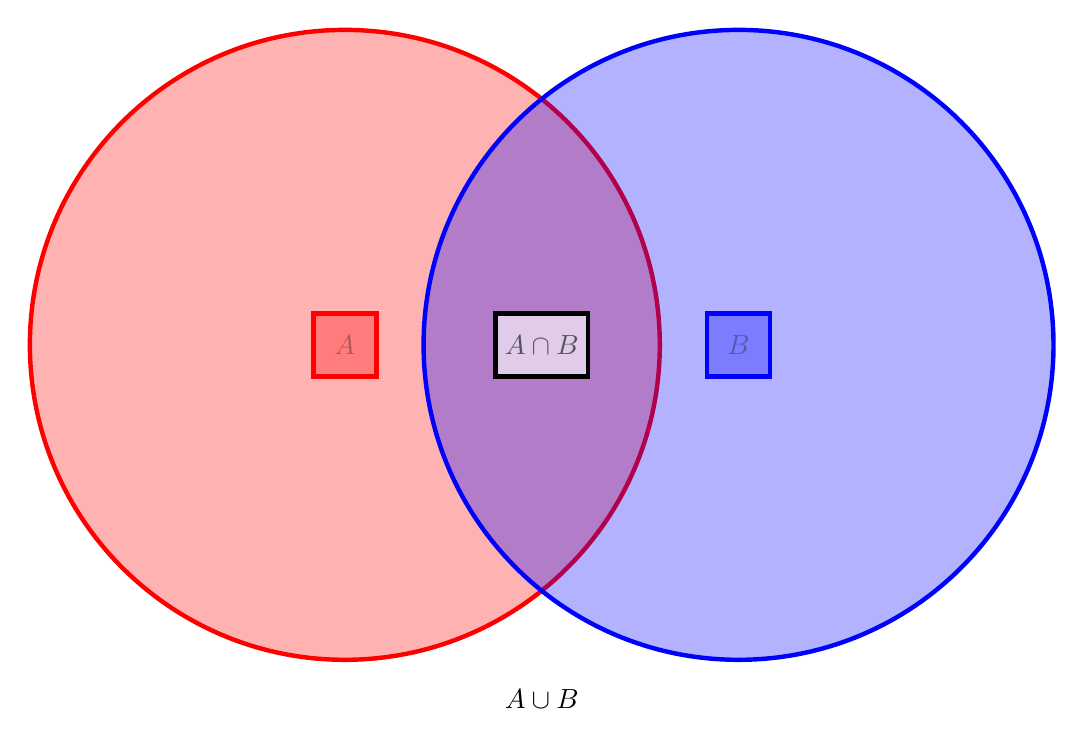
\begin{tikzpicture}
		\draw[ultra thick, draw=red, fill=red, fill opacity=.3] (-2.5,0) circle (4) node[black,draw=red, fill=red, minimum size=0.8cm] {$A$};
		\draw[ultra thick, draw=blue, fill=blue, fill opacity=.3] ( 2.5,0) circle (4) node[black, draw=blue, fill=blue, minimum size=0.8cm] {$B$};

		\draw (0,0) node[ultra thick, draw=black, fill=white, minimum size=0.8cm, fill opacity=0.6] {$A\cap B$} ;

		\draw (0,-4.5) node {$A\cup B$} ;
	\end{tikzpicture}}
	\caption{}
	\label{fig:union}
\end{figure}

Similarly, \textit{set complements} are the set-theoretic negation operator.
Its definition is given as follows:
\begin{define}
	Let $A$ be a set. Then $x\in A^c$ if and only if $x\notin A$.
\end{define}

\cref{fig:not} shows the complement as an operator.
\begin{figure}[h]
\centering
	\resizebox{0.3\linewidth}{!}{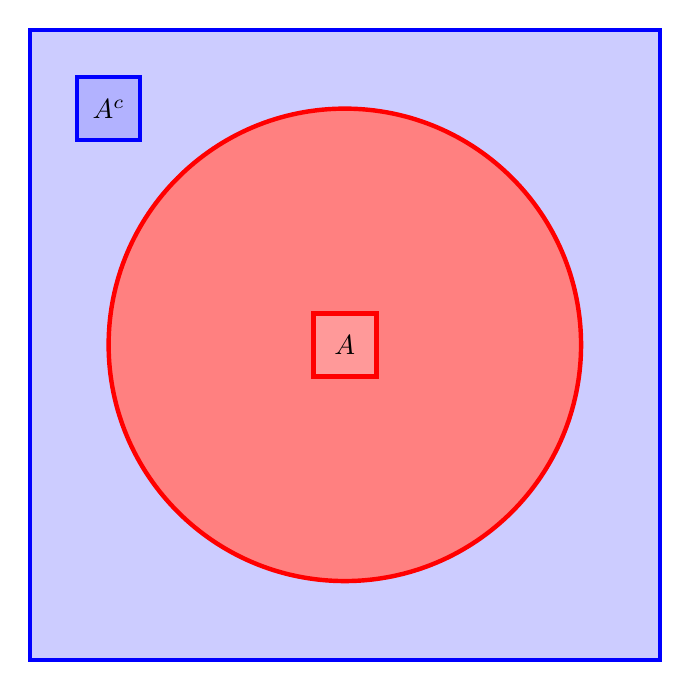
\begin{tikzpicture}
		\draw[ultra thick, draw=blue, fill=blue, fill opacity=.2] (-4,-4) rectangle (4,4);
		\draw[ultra thick, draw=red, fill=red!50] (0,0) circle (3) node[black,draw=red, fill=red!40, minimum size=0.8cm] {$A$};
		\draw (-3,3) node[ultra thick, black, draw=blue, fill=blue!30, minimum size=0.8cm] {$A^c$};
	\end{tikzpicture}}
	\caption{}
	\label{fig:not}
\end{figure}
It should be noted that the complement operator usually requires some assumption of a universal set.
In \cref{fig:not}, the universal set can be represented by the entire area enclosed by the outer blue square.
In most cases, this universal set can be easily identified, but in certain cases where we'd like to specify the universal set in question, we can utilize the \textit{set difference} operator.

When we write $A \setminus B$, the resulting set is the complement in $B$ that is fully contained in $A$.
As such, the definition, very similar to the complement operator, is given as
\begin{define}
	Let $A$ and $B$ be arbitrary sets.
	Then $x\in A\setminus B$ if and only if $x\in A$ and $x\notin B$.\footnotemark
\end{define}
\footnotetext{
	Notice we didn't require $B \subseteq A$.
	This is to means $A\setminus B$ is still a valid statement even if $B$ is entirely not contained in $A$.
	In the cases where $A$ and $B$ are mutually disjoint ($A\cap B=\varnothing$), $A\setminus B = A$.
}

As seen in \cref{fig:set-minus}, the area shaded in red not covered by the blue circle is the result of $A \setminus B$.
\begin{figure}[h]
\centering
\resizebox{0.3\linewidth}{!}{
	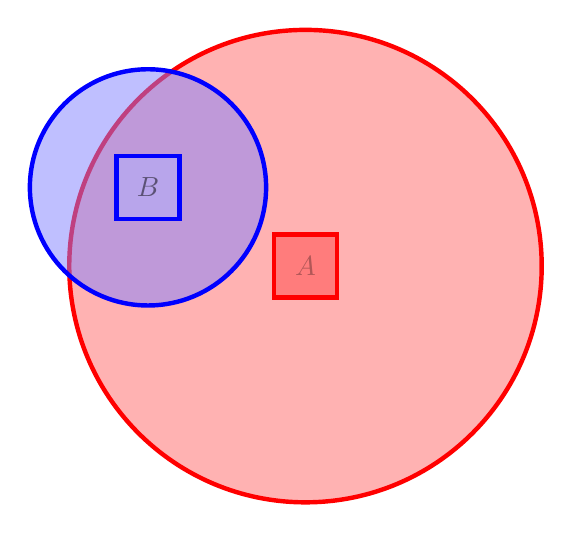
\begin{tikzpicture}
		\draw[ultra thick, draw=red, fill=red, fill opacity=.3] (0,0) circle (3)
			node[black,draw=red, fill=red, minimum size=0.8cm] {$A$};
		\draw[ultra thick, draw=blue, fill=blue!50, fill opacity=0.5] (-2,1) circle (1.5)
			node[black,draw=blue, fill=blue!30, minimum size=0.8cm] {$B$};
	\end{tikzpicture}}
	\caption{$A\setminus B$ defined in red}
	\label{fig:set-minus}
\end{figure}

\subsection{Set Building}
Now that we have a means of talking about and manipulating sets, in this next section, we shall look at examples of sets and ways to construct sets from sets that we already have.

To begin, I've listed in \cref{fig:important-sets} many important sets that we commonly encounter in math.
\begin{figure}[h] \label{fig:important-sets}
	\centering
	\begin{tabular}{| c | m{6cm} |}
		\hline
		Symbol & Definition \\
		\hline
		$\integ$ & Set of all integers \\
		\hline
		$\nat$ & Set of all natural numbers \\
		\hline
		$\real$ & Set of all real numbers \\
		\hline
		$\complex$ & Set of all complex numbers \\
		\hline
		$\rat$ & Set of all rational numbers \\
		\hline
	\end{tabular}
	\caption{}
\end{figure}

The set of integers is the set of all whole numbers (both positive and negative), as many of you hopefully will have seen in previous math classes.
The natural numbers are simply a subset of the integers that consists of only positive (non-zero) integers (e.g 1,2,3,...).\footnote{
	Depending on whom you ask, some people also consider the number 0 a natural number.
	However, as we will find out, this doesn't really change anything (in terms of the structure of the set) and just impacts how we choose to interpret this set.
	In fact, the structure of $\nat$ remains unchanged regardless of where you decide to start it (i.e. taking $\nat$ to be the set of all integers greater than -1,000 would still be equivalent to the standard definition of $\nat$ in the eyes of a set theorist in some sense.)}
We will discuss the rational numbers later on in this section; real and complex numbers in another chapter.

To construct subsets of any existing set, mathematicians commonly employ what is known as a \textit{set-builder}.
As with most other mathematical notation, the symbol we will introduce has very nice translations into English.

Let's say we want to define $A$ as a subset of the integers such that every element is even. We can write
\begin{equation}
	A=\{x\in \integ \mid \textit{x is even}\}
	\label{eq:sample-set-build}
\end{equation}
where $\mid$ translates to the word \textit{given} or \textit{provided}.
Translating equation \eqref{eq:sample-set-build}, we have
\begin{equation}
	A \text{ is equivalent to a set where } x\in \integ \text{ is an element } \textit{provided } x \text{ is even}.
\end{equation}

Often, if the set that we are taking a subset from can be easily inferred, we commonly shorthand equation \eqref{eq:sample-set-build} to
\begin{equation}
	A=\{x \mid \textit{x is even}\}.\footnotemark
\end{equation}
\footnotetext{
	With a bit more mathematical wizardry, we can make this definition of even integers a bit more sophisticated in the following way:
	$$A=\{x \mid (\exists n \in \integ)(x=2n)\}.$$
}

Although originally designed for taking subsets, this notation is sometimes abused to construct sets like the \textit{power set}.
The power set is a powerful tool in set theory, most notably used in the creation of larger sets.
The power set of any set, denoted by $P(A)$, is the set of all subsets of any given set.
Abusing the notation we developed before, we can define
\begin{equation}
	P(A):=\{U \mid U \subseteq A\}.
\end{equation}
Notice, besides the power set itself, there is no set containing all the subsets of $A$ from which we can take $P(A)$ to be a subset of.\footnote{This abuse of notation is commonly what we use to define a class, which is the same as a set in many but certainly not all cases.
We will discuss the differences when we take a more rigorous approach to set theory.}
%TODO: add definition of := somewhere

If we let $(x,y):=\{x,\{y\}\}$,\footnote{When we define sets more rigorously, we want every object we work with to be a \textit{set}, hence the weird definition of an ordered pair.} we can also define the set of all \textit{ordered pairs} as a set of sets, where if $X$ and $Y$ are sets, then
\begin{equation}
	X\times Y := \{(x,y) \mid x \in X \text{ and } y \in Y\}.
\end{equation}
where $(x,y)$ is the set defined above and $X\times Y$ is the \textit{cartesian product} of $X$ and $Y$, or the set of all ordered pairs of elements in $X$ followed by elements in $Y$.

We can, in theory, repeat the process of taking Cartesian products to get sets of ordered triples, quadruples, or more generally, ordered \textit{$n$-tuples}.
As $n$ gets large, to help facilitate with notation, let $\mathcal C$ be a collection of sets.
Then to take an $n$ product of sets in $\mathcal C$, we first assign each natural number $i \le n$ to a unique element in $\mathcal C$.
This makes precise the statement \textit{$i$th set in $\mathcal C$}, which we take to mean the element $C_i\in mathcal C$ with the index $i$.
With this, we can denote the $n$-product as
\begin{equation}
	\prod_{C_i \in \mathcal C} C_i := C_1 \times C_2 \times ... \times C_n.
\end{equation}
To denote each $n$-tuple we write $(c_i)_{i\le n}$, were each $c_i\in C_i$ is the $i$th element in the tuple.

Note, we might have $C_m=C_n$ for $m\neq n$, for example, if we take the product of $n$ copies of $C$, then the collection $\mathcal C$ has one element and $C_i=C_j$ for all $i,j \le n$.
Thus, this product
\begin{equation}
	\underbrace{C \times ... \times C}_n = \prod_{i \le n} C_i
\end{equation}
If the product consists of a single set, sometimes, we simplify the notation by simply writing $\prod_{i\le n} C$, or $C^n$.

To generalize this to infinite products, observe in the finite case, if we let $I$ be the collection of indices, $I$ is the set
\begin{equation}
	I:=\{k \in \nat \mid k \le n\}.
\end{equation}
To generalize to infinite products, we simply allow this indexing set $I$ be arbitrary.
Then like before, if we assign each element $i \in I$ to a unique element in $\mathcal C$, we denote the product $\prod_{i \in I} C_i$ as the set of infinite tuples $(c_i)_{i \in I}$ where $c_i \in C_i$ for each $i \in I$.
In general, we will refer infinite tuples as simply a \textit{sequence} when we take the indexing set to be $\nat$.\footnote{We will see that infinite indexing sets are not all created equal: in particular a collection indexed by $\real$ results in a significantly different product than a collection indexed by $\nat$. We will see the reasons for why in a later section.}
Like in the finite case, when we take the infinite product of the same set, we denote this product as $C^I$ where, $I$ is the indexing set.

Let's also denote a very special type of set by the following definition:
\begin{define} \label{def:singleton}
	Let a \textit{singleton} denote any one-point-set (i.e. sets of the form $\{x\}$).
\end{define}
